\chapter{Support Vector Machines}
Il percettrone, sebbene sia estremamente semplice, riesce ad impara solo funzioni di separazione lineari. Le reti neurali multistrato invece riescono anche ad apprendere funzioni di separazione non lineari complesse ma con
difficoltà di addestramento avendo molti minimi locali e tanti pesi. Le Support Vector Machines (\textbf{SVM}) presentano un algoritmo di apprendimento efficiente e imparano funzioni di
separazione non lineari complesse.
\section{Una visione alternativa della regressione logistica}
Le \textit{Support Vector Machine} possono essere viste come una versione alternativa della regressione logistica. In particolare prendiamo in considerazione la funzione sigmoide:
\[h_\theta(x) = \frac {1} {1 + e^{-z}}\]
\begin{nota}
Ricordiamo che si vuole intendere $z = \Theta^T x$
\end{nota}
Prendiamo in considerazione la regressione logistica e la sua relativa funzione di costo:
% <![CDATA[
\begin{align*}
J(\theta) &= -{1 \over m} \sum_{i=1}^m \left( y^{(i)}\,log(h_\theta(x^{(i)}) + (1-y^{(i)})\,log(1 - h_\theta(x^{(i)})) \right) \\
    &= -{1 \over m} \sum_{i=1}^m \left( y^{(i)}\,log(\frac {1} {1 + e^{-\theta^T x}}) + (1-y^{(i)})\,log(1 - \frac {1} {1 + e^{-\theta^T x}}) \right)
\end{align*} %]]>
Dove ogni esempio nel DataSet contribuisce alla funzione di costo:
\[-y\,log(\frac {1} {1 + e^{-z}}) - (1-y)\,log(1 - \frac {1} {1 + e^{-z}})\]
Andando a modificare tale funzione di costo avremo un problema più semplice da risolvere. In particolare le SVM sfruttano una semplificazione della funzione di costo indicata (\ref{Fig:SVMCosty1} e \ref{Fig:SVMCosty0}).
\begin{figure}[!htb]
   \begin{minipage}{0.48\textwidth}
     \centering
     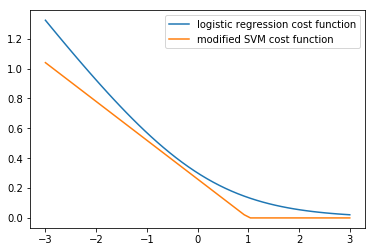
\includegraphics[width=.7\linewidth]{img/costFunSVMy1.png}
     \caption{Funzione di costo per SVM con y = 1}\label{Fig:SVMCosty1}
   \end{minipage}\hfill
   \begin{minipage}{0.48\textwidth}
     \centering
     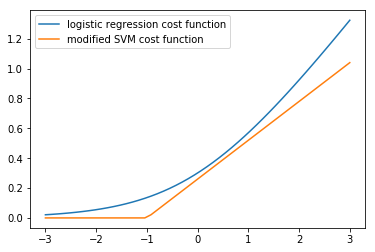
\includegraphics[width=.7\linewidth]{img/costFunSVMy0.png}
     \caption{Funzione di costo per SVM con y = 0}\label{Fig:SVMCosty0}
   \end{minipage}
\end{figure}
Da cui si evincono le funzioni di costo per le SVM: $Cost_0(\Theta^Tx)$ per le predizioni di $y=0$ e $Cost_1(\Theta^Tx)$ per le predizioni di $y=1$.
\subsection{Funzione di costo per le SVM}
Ricordiamo che nella funzione logistica possiamo inserire il parametro di regolarizzazione seguendo la funzione di costo:
\[J(\theta) = {1 \over m} \sum_{i=1}^m \left( y^{(i)}\,(-log(h_\theta(x^{(i)}))) + (1-y^{(i)})\,(-log(1 - h_\theta(x^{(i)}))) \right) + {\lambda \over 2m } \sum_{j=1}^n \theta_j^2\]
Che si può riscrivere nella forma di parametrizzazione:
\[A + \lambda B\]
Da essa ricaviamo una prima forma di funzione di costo per le SVM sostituendo semplicemente i termini di costo:
\[J(\theta) = {1 \over m} \sum_{i=1}^m \left( y^{(i)}\,cost_1(z) + (1-y^{(i)})\,cost_0(z) \right) + {\lambda \over 2m } \sum_{j=1}^n \theta_j^2\]
Notiamo però alcuni accorgimenti che possiamo attuare per cambiare la notazione pur facendo rimanere inalterata la logica:
\begin{itemize}
    \item Rimuove il parametro $\frac{1}{m}$ non ha effetto sulla minimizzazione poiché rimane sempre costante.
    \item Inserendo un termine $C = \frac{1}{\lambda}$ possiamo scrivere che $A + \lambda B = CA+B$.
\end{itemize}
Da cui si evince la seguente funzione di costo (equivalente logicamente alla precedente):
\[J(\theta) = C \sum_{i=1}^m \left[ y^{(i)}\,cost_1(\theta^T x^{(i)}) + (1-y^{(i)})\,cost_0(\theta^T x^{(i)}) \right] + {1 \over 2 } \sum_{j=1}^n \theta_j^2\]
% \begin{figure}[H]
%     \centering
%     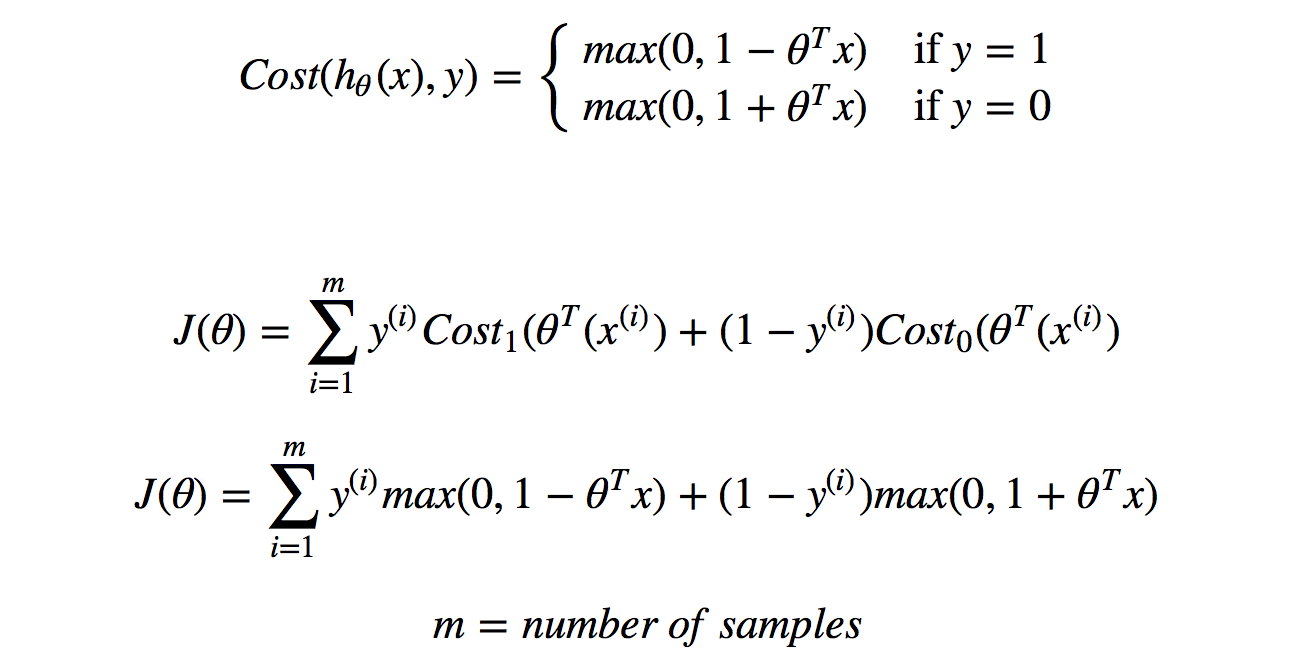
\includegraphics[width=1\textwidth]{img/costFunctionSVM.png}
% \end{figure}
% Su cui possiamo anche inserire un parametro di regolarizzazione:
% \begin{figure}[H]
%     \centering
%     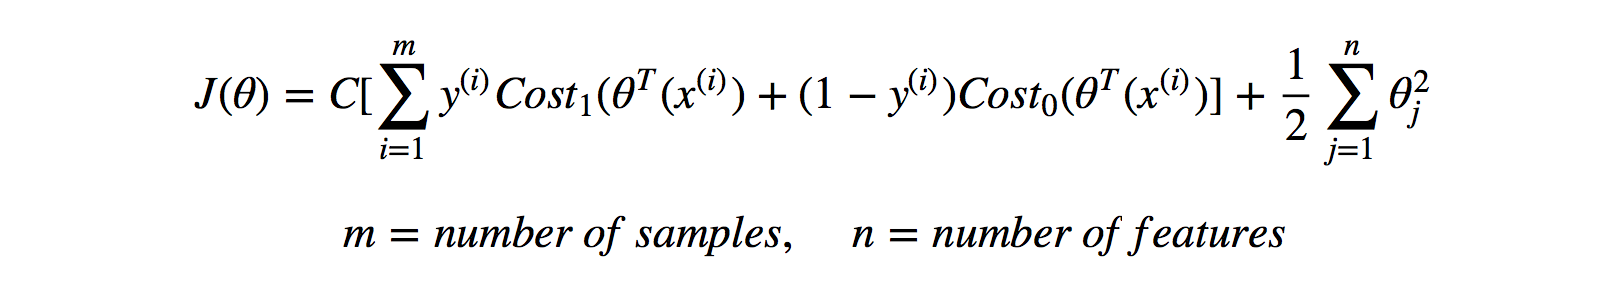
\includegraphics[width=1\textwidth]{img/costFunctionSVM2.png}
% \end{figure}
Per cui prendiamo in considerazione la seguente ipotesi per le SVM:
  \[h_\theta(x) =
    \begin{cases}
      1& \iff \Theta^Tx \geq 0 \\
      0& Altrimenti
    \end{cases}
  \]
% \begin{figure}[H]
%     \centering
%     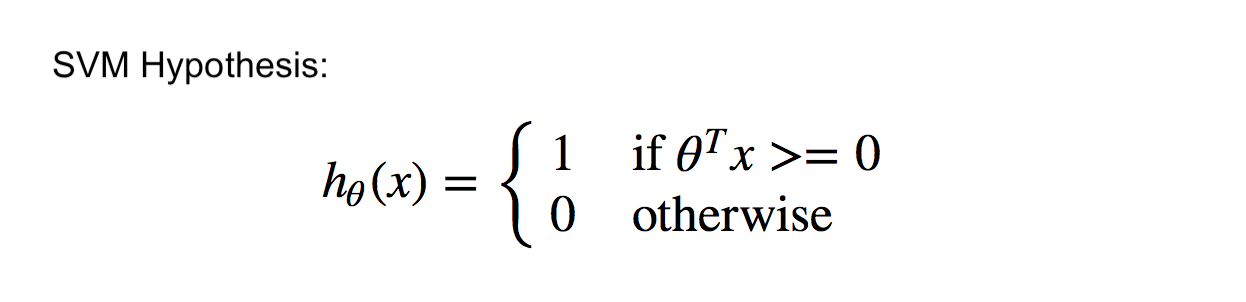
\includegraphics[width=1\textwidth]{img/SVMHypo.png}
% \end{figure}
\section{Margine e confine decisionale}
\begin{figure}[H]
    \centering
    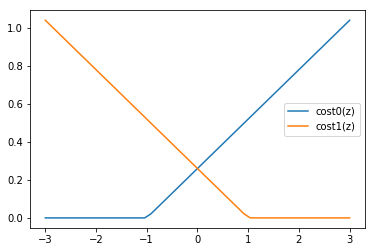
\includegraphics[width=1\textwidth]{img/cost-plots-SVM.png}
    \caption{SVM funzioni di costo}
    \label{Fig:SVMCostPlots}
\end{figure}
Notando la figura \ref{Fig:SVMCostPlots} forniamo le seguenti osservazioni:
  \[y =
    \begin{cases}
      1& \implies \Theta^Tx \geq 1 \,\,\,\mbox{ NON basta $\geq$ 0 }\\
      0& \implies \Theta^Tx \leq -1 \,\,\,\mbox{ NON basta < 0 }
    \end{cases}
  \]
\subsection{Minimizzazione della funzione di costo}
Lasciando che il parametro \[C = \frac{1}{\lambda} \to \infty\]
Per minimizzare la funzione di costo allora:
\[\sum_{i=1}^m \left[ y^{(i)}\,cost_1(\theta^T x^{(i)}) + (1-y^{(i)})\,cost_0(\theta^T x^{(i)}) \right] \to 0\]
In particolare si deve far si che:
  \[y =
    \begin{cases}
      1& \implies Cost_1(\Theta^Tx) = 0\\
      0& \implies Cost_0(\Theta^Tx) = 0 
    \end{cases}
  \]
  \begin{esempio}
Se avessimo una predizione $y=1$ allora dovremo rifarci alla funzione $Cost_1(\Theta^Tx)$, tale per cui se il nostro input $x$ sia tale che $\Theta^Tx < 1$ allora il costo stesso fornito dalla funzione tenderebbe a $\infty$. Quest'ultimo ci avvertirebbe che la nostra ipotesi non è sicuramente adatta alla tipologia di predizione considerata.
\end{esempio}
Seguendo quindi questa intuizione possiamo descrivere il tutto come:
\[min_\theta J(\theta) = min_\theta {1 \over 2 } \sum_{j=1}^n \theta_j^2\]
% <![CDATA[
\begin{align*}
\theta^Tx^{(i)} &\geq 1 \text{, if } y^{(i)}=1 \\
\theta^Tx^{(i)} &\leq -1 \text{, if } y^{(i)}=0
\end{align*} %]]>
Dalla precedente osservazione possiamo anche notare che basterebbe $\Theta^Tx \geq 0$ per classificare un esempio come positivo. Ora sicuramente i lettori si staranno ponendo la seguente domanda: \textit{"Mario, ma allora perché stiamo ponendo $\Theta^Tx \geq 1$?"}. La risposta alla domanda riguarda la differenza stessa tra la \textit{regressione logistica} e le \textbf{Support Vector Machine}, ovvero: quest'ultime preservano un comportamento chiamato \textbf{margine}. Esso si ottiene principalmente dalla \textbf{minimizzazione della funzione di costo}, in particolare si raggiunge un \textbf{decision boundary} molto interessante tale per cui il \textbf{margine} sia il più grande possibile. In particolare ricordiamo che la minimizzazione della funzione di costo ha il compito di trovare i valori di $\theta$ più bassi, in dettaglio al variare di tali valori vari anche il confine decisionale.
\begin{figure}[H]
    \centering
    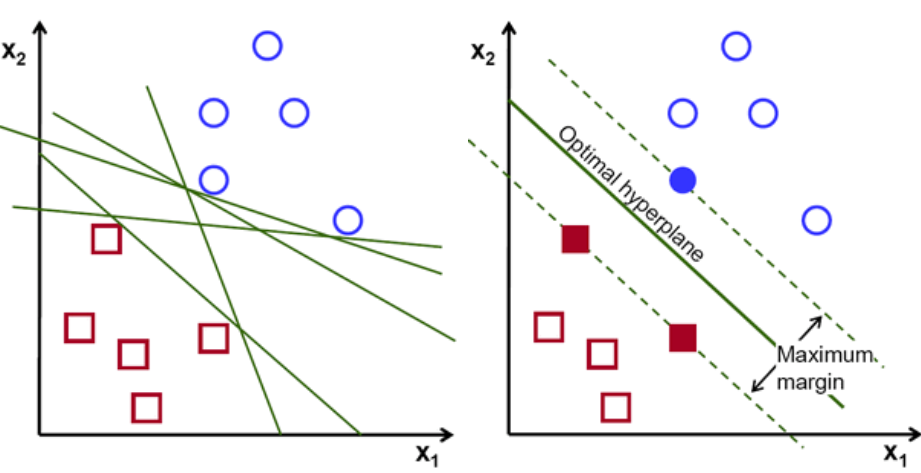
\includegraphics[width=1\textwidth]{img/margin.png}
\end{figure}
\begin{definizione}
  La SVM è un classificatore di margini di grandi dimensioni.
\end{definizione}
Dando più \textit{"priorità"} al parametro $A$ mediante $C$ avremo:
\begin{figure}[H]
    \centering
    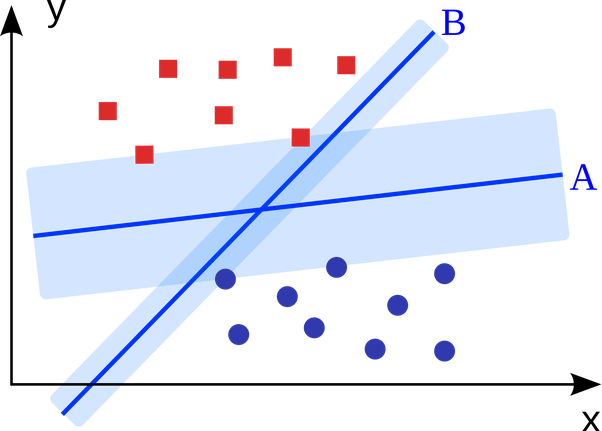
\includegraphics[width=0.7\textwidth]{img/fig-4-large-margin-decision-boundary.png}s
\end{figure}
\subsubsection{L'effetto del Parametro C}
Il parametro $C$ può essere visto come $\frac{1}{\lambda}$. In particolare un valore piccolo di C garantisce che i valori anomali (\textit{outliers}) vengano trascurati e che venga determinata la migliore approssimazione per il margine. 
\begin{figure}[H]
    \centering
    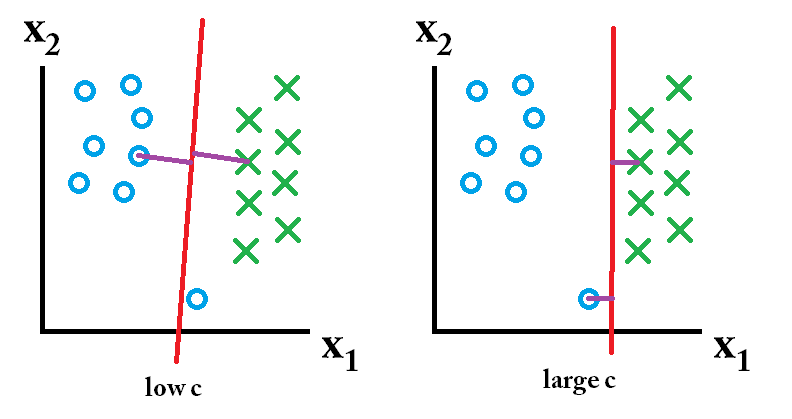
\includegraphics[width=1\textwidth]{img/fig-5-effect-of-regularization.png}
\end{figure}

\section{Kernel: un modo per classificare ipotesi non lineari}
Le \textit{Support Vector Machine} riescono anche a classificare funzioni \textbf{non lineari complesse}. Un modo per farlo è quello di trovare una serie di caratteristiche polinomiali complesse: facciamo corrispondere ogni vettore di input $x$ a un nuovo vettore $f$ di valori di caratteristiche.
  \[h_\theta(x) =
    \begin{cases}
      1& \iff \Theta^Tf \geq 0 \\
      0& Altrimenti
    \end{cases}
  \]
\begin{figure}[H]
    \centering
    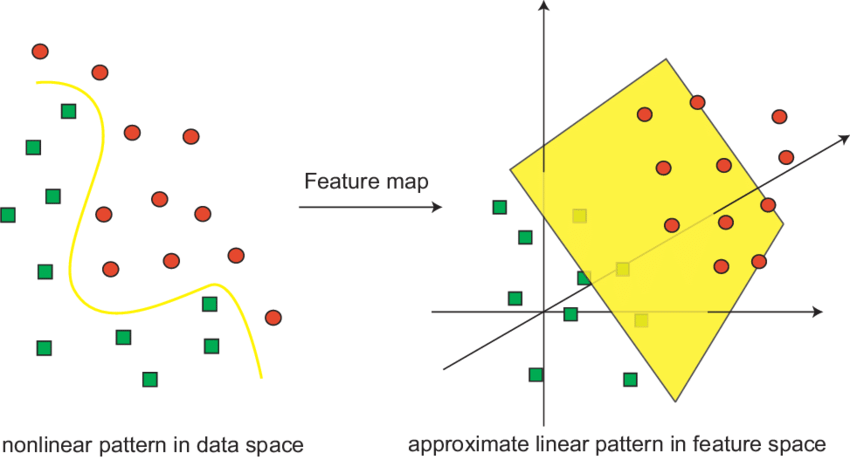
\includegraphics[width=1\textwidth]{img/linear_nonLinear.png}
\end{figure}
\begin{definizione}
  Se i dati sono rimappati in uno spazio che ha un numero sufficiente di dimensioni, saranno sempre linearmente separabili.
\end{definizione}
\begin{esempio}
  Immaginiamo di voler trovare il miglior separatore lineare per la funzione in figura \ref{NonLinearFunction}:
  \begin{figure}[H]
    \centering
    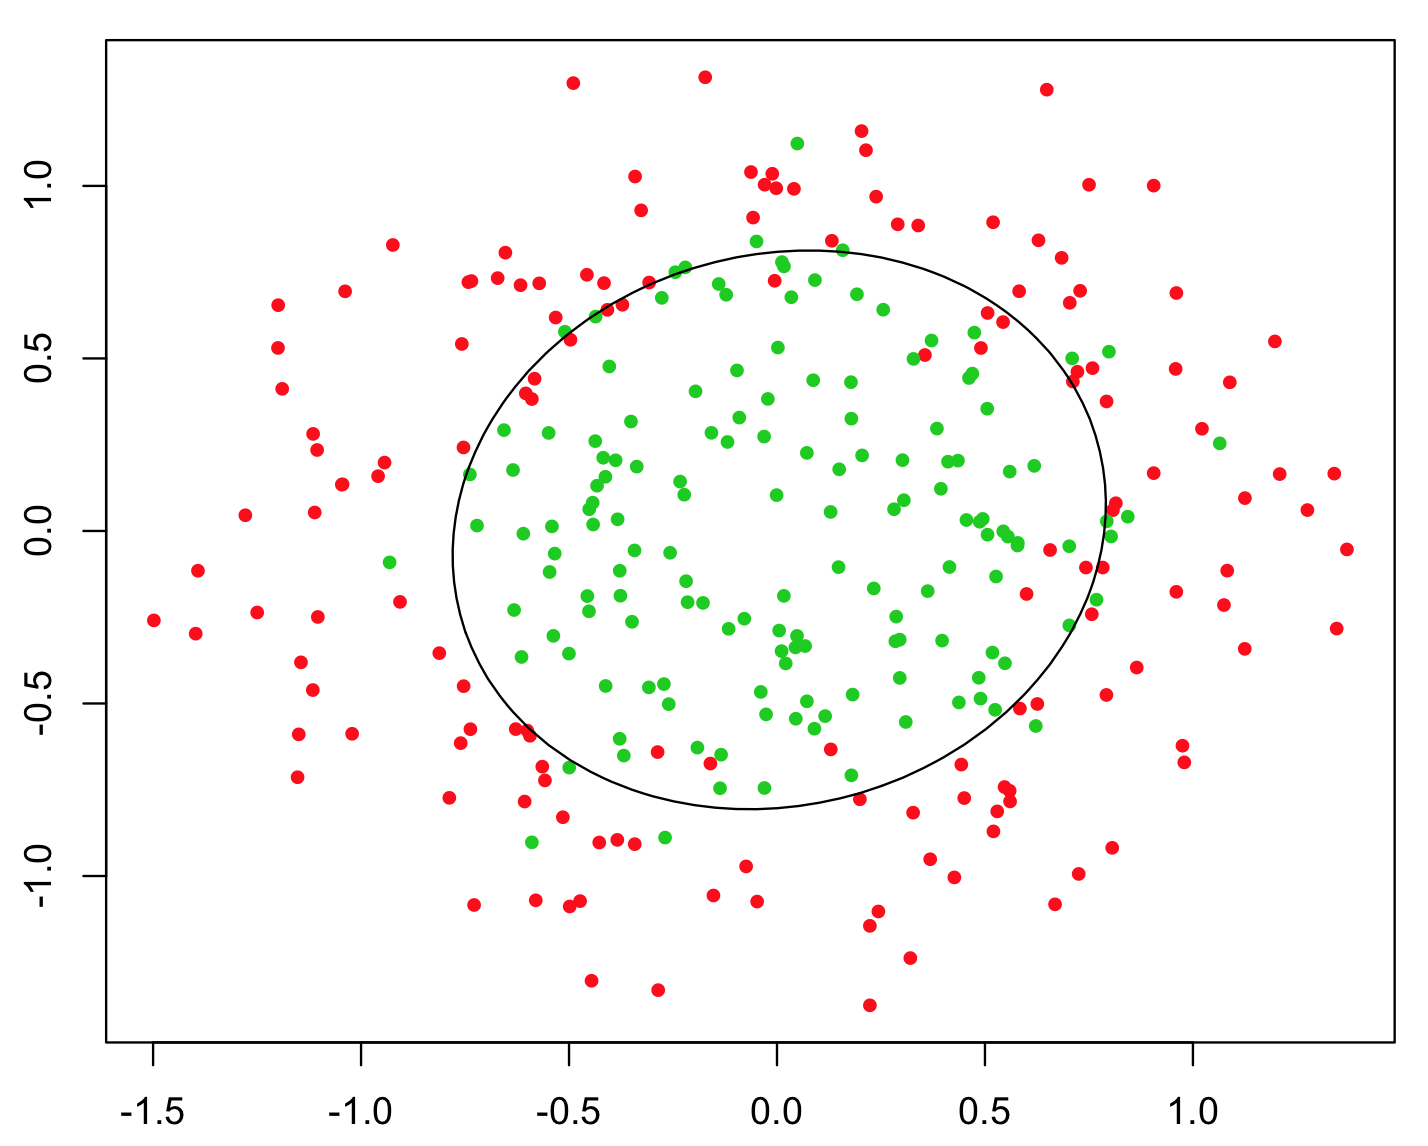
\includegraphics[width=0.7\textwidth]{img/nonLinearFunction.png}
    \caption{Dataset non linearmente separabile}
    \label{NonLinearFunction}
\end{figure}
Per farlo prendiamo in considerazione la seguente ipotesi:
\[h_\theta(x) =
    \begin{cases}
      1& \iff \theta_0 + \theta_1x_1 + \theta_2x_2 + 
      \theta_3x_1x_2 + \theta_4x^2_1 \dots \geq 0 \\
      0& Altrimenti
    \end{cases}
  \]
  Essendo l'insieme di dati non linearmente separabile, sfruttiamo una mappatura mediante un insieme di caratteristiche:
  \[f_1 = x_1,\,\,\,f_2 = x_2,\,\,\,f_3 = x_1x_2, \,\,\, f_4 = x_1^2 \,\,\,\dots\]
  Da cui deriviamo la nuova ipotesi \textbf{linearmente separabile}:
  \[h_\theta(x) =
    \begin{cases}
      1& \iff \theta_0 + \theta_1f_1 + \theta_2f_2 + 
      \theta_3f_3 + \theta_4f_4 \dots \geq 0 \\
      0& Altrimenti
    \end{cases}
  \]
\end{esempio}
\subsection{Creazione delle caratteristiche}
Ora la domanda sorge spontanea: \textit{"Mario, ma come facciamo a trovare le features per eseguire una mappatura?"}. Per rispondere a questa domanda dobbiamo introdurre i \textbf{vettori di supporto}: punti sull'estremità del margine del separatore lineare che hanno il compito di punti di riferimento (fig.\ref{supportVector}). \textbf{Per ognuno di questi punti esiste una nuova feature}.
\begin{figure}[H]
    \centering
    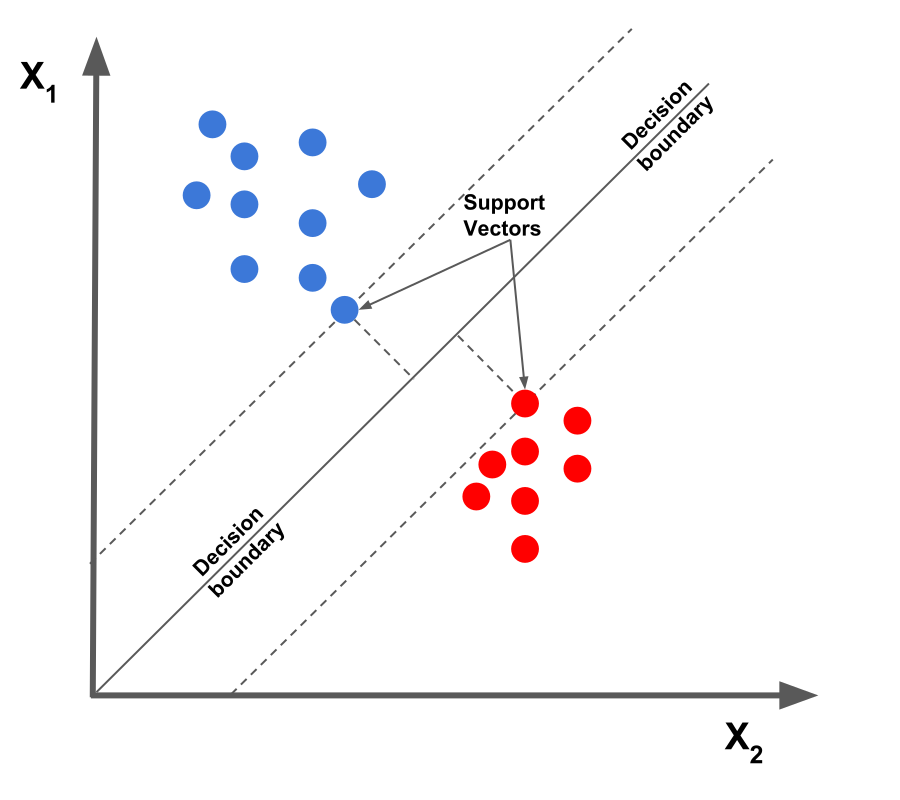
\includegraphics[width=0.7\textwidth]{img/supportVector.png}
    \caption{Vettori di supporto}
    \label{supportVector}
\end{figure}
\begin{definizione}
  Dato un vettore $x$ e un insieme di vettori di supporto $l^{(i)}$, definiamo le caratteristiche $f_i$ come:
  \[f_i = similarity(x,l^{(i)}) = k(x,l^{(i)})\]
\end{definizione}
Le \textbf{funzioni kernel} esprimono quindi la \textit{"somiglianza"} tra un esempio $x$ e un vettore di supporto $l^{(i)}$. In particolare la funzione kernel più utilizzata è quella \textbf{Gaussiana}:
  \[ exp\left(-\frac{\lVert x - l^{(k)}\lVert^2}{2\sigma^2}\right) = \left(-\frac{\sum_j(x_j-l_j^{(k)})^2}{2\sigma^2}\right)\]
\begin{nota}
$\lVert x - l^{(i)} \lVert$ è la distanza euclidea tra due punti.
\end{nota}
Da tale funzione kernel possiamo notare caratteristiche importanti nel calcolo del \textbf{separatore ottimo}:
  \[f_n \approx
    \begin{cases}
      1& \iff x \approx l^{(k)} \\
      0& Altrimenti
    \end{cases}
  \]
  \begin{nota}
  \[x \approx l^{(k)} \implies  exp\left(-\frac{0^2}{2\sigma^2}\right)  \approx 1\]
  \[x \neq l^{(k)} \implies  exp\left(-\frac{\infty}{2\sigma^2}\right)  \approx 0\]
  \end{nota}
\begin{esempio}
  Sia $\Theta = [-0.5, 1, 1, 0]$ e siano 3 i valori di vettori di supporto $l^{(k)}$. Definiamo l'ipotesi come:
  \[h_\theta(x) =
    \begin{cases}
      1& \iff \theta_0 + \theta_1f_1 + \theta_2f_2 + 
      \theta_3f_3 \geq 0 \\
      0& Altrimenti
    \end{cases}
  \]
  Se avessimo $x \approx f_1$ avremo:
  \[f_1 \approx 1,\,\,\,f_2 \approx 0,\,\,\,f_3 \approx 0\]
  Da cui si deriva che:
  \[\theta_0 + \theta_1 = -0.5+1 = 0.5 \implies h_\theta(x) = 1\]
\end{esempio}
\subsection{Creazione dei vettori di supporto}
Abbiamo spiegato che i vettori di supporto sono punti di riferimento posti al confine del margine dato dal separatore. Ora i cari lettori sicuramente si porgeranno la seguente domanda: \textit{"Mario, ma questi vettori di supporto come li possiamo creare se ancora non conosciamo a priori né il separatore né il corrispettivo margine?"}. 
\begin{definizione}
  Preso un DataSet con esempi sia positivi che negativi. Per ogni esempio si va a creare un corrispettivo punto di riferimento nella medesima posizione. In particolare, preso un dataset:
  \[{(x_1, y_1) \dots (x_n, y_n)}\]
  Si avranno:
  \[{(x_1 = l^{(1)}) \dots (x_n, l^{(n)})}\]
\end{definizione}
Questo è abbastanza utile poiché quando si riceverà un esempio \textbf{non} catalogato possiamo avere come punti di riferimento le coordinate degli esempi già analizzati in precedenza. Ovvero:
\[f_n = similarity(x_{new}, l^{(n)})\,\,\,\,\, \forall n \implies f_n = [f_1 \dots f_n]\]
Quindi si applica la funzione kernel in relazione ad ogni possibile vettore di supporto. \\ Allo stesso tempo, per creare una mappatura di tutti gli elementi presente nel dataset eseguiamo la medesima procedura:
\[x_i \implies 
    f = \begin{bmatrix}
           f_{1} \\
           f_{2} \\
           \vdots \\
           f_{i} = 1 \\
           \vdots \\
           f_{n}
         \end{bmatrix} \]
In questa specifica situazione notiamo un fattore importante: esisterà $f_{i} = 1$ per $x_i$ poiché sarà relativo al vettore di supporto $l^{(i)}$.
\subsection{Kernel e Funzione di costo}
La funzione di costo, prese in considerazione le features calcolate, si può riscrivere come:
\[min_\theta \, C \sum_{i=1}^m \left[ y^{(i)}\,cost_1(\theta^T f^{(i)}) + (1-y^{(i)})\,cost_0(\theta^T f^{(i)}) \right] + {1 \over 2 } \sum_{j=1}^m \theta_j^2\]
\section{Scelta dei Kernel}
Le funzioni kernel per la creazione delle \textit{features} sono diverse, in particolare le più utilizzate sono:
\begin{itemize}
    \item \textbf{Linear Kernel}: equivalente a non usare una funzione kernel, con essa possiamo quindi sfruttare le funzionalità basilari di una SVM che riesce solo a produrre una classificazione lineare. L'utilizzo di tale kernel presuppone la \textbf{non} creazione di vettori di supporto. Essa viene spesso utilizzata quando il numero di esempi nel DataSet è piccolo ma il numero di classificazioni è grande.
    \[\theta_0\,x_0 + \theta_1\,x_1 + \theta_2\,x_2 + \theta_3\,x_3 + \cdots \geq 0\]
    \item \textbf{Gaussian Kernel}: Utilizzato quando il numero di esempi è elevato e il numero di classificazioni è basso (es. classificazione binaria).
\end{itemize}
\begin{definizione}
  Tutti i kernel sfruttati dalle SVM devono soddisfare il \textbf{Torema di Mercer} per essere sicuri che l'ottimizzazione delle SVM non diverga.
\end{definizione}
\begin{nota}

Esiste un altro kernel meno utilizzato: \textbf{Polynomial Kernels}:
\[k(x, l) = (x^T l + constant)^{degree}\]
\end{nota}
\section{Regressione Logistica vs SVM}
Sia $n$ il numero di classificazioni in un DataSet e $m$ il numero di esempi. 
\begin{itemize}
    \item Se $n >> m$ allora possiamo sfruttare la regressione logistica o una SVM con Kernel lineare. Questo poiché se avessimo tante caratteristiche differenti in un dataset molto piccolo allora non avremo a disposizione abbastanza dati per creare un adattamento ad una funzione non lineare complessa.
    \item se $n$ è  piccolo e $m$ è intermedio allora possiamo sfruttare le SVM con Kernel Gaussiano.
    \item Se $m >> n$ allora possiamo creare manualmente più classificazioni per poi utilizzare la regressione logistica o la SVM con kernel lineare.
\end{itemize}
% \section{Altro}
% Viene quindi ripreso comunque il concetto di \textit{separazione lineare} ma con una scelta efficiente dell'iperpiano, trovando il \textbf{miglior iperpiano separatore}, per classificare un insieme di punti linearmente separabili, trovando un vettore di pesi $W$ per separare bene le istanze. Si usa la cosiddetto \textbf{teoria statistica dell’apprendimento} che dice che tra tutti gli iperpiani che possiamo usare per separare due classi si sceglie quello che sia in grado di etichettare meglio nel futuro. L'intuizione è quella di prendere un iperpiano ottimo rispetto alla misura della distanza minima che si ha tra gli esempi, si guardano quindi tutti i punti del training set e cerco di piazzare in mezzo l'iperpiano, in modo che intorno ad esso ci sii massima ampiezza. Tale ampiezza è detta margine (volendo che sia massima la distanza minima tra tutti i punti). SVM usa questa teoria per trovare l'iperpiano ``migliore'' in base a
% questi calcoli probabilistici. 




% % magari pic
% Non si parla quindi più di neuroni.\\
% e riuscissimo a separare i dati con un largo margine
% avremmo ragione di credere che il classificatore (ovvero l'iperpiano stesso) sia
% ``più robusto'' tanto da avere una migliore generalizzazione (assunto che i
% punti siano generati da una certa regola).
% Quando arriva quindi un nuovo punto, generato con la stessa regola degli altri,
% sarà sicuramente classificato correttamente, una volta scelto l'iperpiano.\\
% Ci serve quindi la separabilità delle istanze, serve quindi che la funzione
% generatrice sia linearmente separabile.
% \begin{definizione}[dimensione di Vapnik-Cervonenkis]
%   Con la teoria statistica dell'apprendimento si dimostra che più allarghiamo il
%   margine meglio l’iperpiano generalizza, raggiungendo la dimensione di
%   Vapnik-Cervonenkis (VC).\\
%   Prese tutte le funzioni che generano il training set si produce la VC che
%   esprime quanto è difficile sbagliare sulle ipotesi future in base alla scelta
%   dell'iperpiano.
% \end{definizione}
% Dobbiamo quindi scrivere un algoritmo per trovare l'iperpiano di separazione di
% massimo margine. In input si hanno le istanze etichettate e in output un
% vettore che identifica l'iperpiano.\\
% Viene usata una notazione matematica che prevede che, preso un insieme di punti
% di training:
% \[S = \{(x_1, y_1), (x_2, y_2),\ldots, (x_n, y_n)\}\]
% a ogni vettore $x_i$ associo la classe di appartenenza $y_i$ (con un etichetta
% non booleana):
% \[y_i\in\{-1,+1\}\]
% Ho i punti linearmente separabili:
% \[
%   \begin{cases}
%     \langle w, x_i\rangle + b >0 &\mbox{se }y_i=+1\\
%     \langle w, x_i\rangle + b <0 &\mbox{se }y_i=-1\\
%   \end{cases}
% \](quindi l'iperpiano separa positivi e negativi)\\
% che scritto in un solo vincolo diventa:
% \[y_i(\langle w, x_i\rangle + b )>0,\,\,\, i=1,\ldots, n\]
% Si ha che $w$ mi dirà quanto è inclinato il piano mentre $b$ è la distanza tra
% l'origine e il piano (quindi queste due variabili identificano i vari iperpiani
% possibili tra cui cercare il ``migliore'' ovvero quello che separa meglio punti
% positivi e negativi).\\
% Ci si sposta quindi dalla geometria visualizzabile all'algebra lineare.\\
% L'ipotesi quindi tra $w$ e $b$ è una funzione che prende il segno di $<langle
% w, x\rangle+b$ per associare l'etichetta:
% \[h_{w, b}(x)=sgn(\langle w, x\rangle+b)\]
% Date $d_-$ e $d_+$ le distanze tra l’iperpiano separatore e il punto positivo e
% negativo più vicino definiamo:
% \begin{itemize}
%   \item margine funzionale
%   \item margine geometrico
% \end{itemize}
% \begin{definizione}
%   Definiamo il \textbf{margine funzionale} di un punto $(x_i, y_i)$ rispetto
%   all'iperpiano $(w, b)$ come:
%   \[\hat{\gamma}=y_i\cdot(\langle w, x_i\rangle+b)\]
%   e quindi il \textbf{margine funzionale} dell'iperpiano rispetto al training
%   set $S$ è definito come:
%   \[\hat{\rho}=\min_{i=1,\ldots, n}\hat{\gamma_i}\]
% \end{definizione}
% Si hanno quindi due casistiche:
% \begin{enumerate}
%   \item se si ha un punto $x_i$ tale che $y_i=+1$, perchè il margine funzionale
%   sia grande è necessario che la quantità
%   $\langle w, x_i\rangle+b$ abbia un grande valore positivo
%   \item se si ha un punto $x_i$ tale che $y_i=-1$, perchè il margine funzionale
%   sia grande è necessario che  la quantità
%   $\langle w, x_i\rangle+b$ abbia un grande valore negativo
% \end{enumerate}
% \begin{definizione}
%   Se $\hat{\gamma}_i>0,\forall \mbox{classificazione} i$ la classificazione è
%   approvata in quanto le classi sono linearmente separabili e l'iperpiano
%   $(w, b)$ separa effettivamente le classi
% \end{definizione}
% Si ha quindi che un ampio margine funzionale fornisce probabilità sulla qualità
% della previsione anche se l'uso del solo $\hat{\gamma}$ può essere problematico
% in quanto il margine funzionale non è invariante rispetto a un iperpiano
% ``riscalato''. Analizziamo meglio quest'aspetto.\\
% Per come è stato scelto il classificatore $f$ se si scala l'iperpiano:
% \[(w, b)\to(c\cdot w, b)\]
% si ottengono:
% \begin{itemize}
%   \item lo stesso iperpiano, ovvero lo stesso luogo di punti
%   \item la stessa funzione di decisione, visto che quest'ultima dipende solo dal
%   segno di $\langle w, x\rangle+b$, con il segno che può essere invertito se
%   $c<0$ 
% \end{itemize}
% ma dato che il margine funzionale viene moltiplicato per $c$ non possiamo usarlo
% come distanza di un punto dall’iperpiano, perché non è invariante rispetto alla
% scala.\\
% Bisogna ora studiare la distanza $d$ del punto $x$ dall'iperpiano. Si ha quindi:
% \[d = \frac{\sum_{i=1}^n w_i\cdot x_i+v}{\norm{w}}=\frac{\langle w,
%     x_i\rangle +b}{\norm{w}} \]
% Quindi:
% \begin{definizione}
%   Definiamo il \textbf{margine geometrico} di un punto $(x_i, y_i)$ rispetto
%   all'iperpiano $(w, b)$ come:
%   \[\gamma_i=\frac{y_i\cdot(\langle w, x_i\rangle+b)}{\norm{w}}\]
%   e quindi il \textbf{margine geometrico} dell'iperpiano rispetto al training
%   set $S$ è definito come:
%   \[\rho=\min_{i=1,\ldots, n}\gamma_i\]
% \end{definizione}
% \begin{definizione}
%   Se $\gamma_i>0,\forall \mbox{classificazione} i$ la classificazione è
%   approvata analogamente a quanto detto per il margine funzionale.
% \end{definizione}
% ato un punto positivo/negativo il margine geometrico rappresenta la sua
% distanza geometrica dall'iperpiano. quindi il margine geometrico rende meglio
% l'idea della distanza di un punto sa un iperpiano in $\mathbb{R}^n$.\\
% Inoltre si ha che \textbf{i margine geometrico è invariante rispetto alla scala
%   di $w$} e quindi possiamo ``riscalare'' l'iperpiano senza cambiamenti, non
% variando il margine.\\
% Dalla formula notiamo che, posto $\norm{w}=1$ si ``riscala'' l'iperpiano $(w, b)$:
% \[(w, b)\to\left(\frac{w}{\norm{w}},\frac{b}{\norm{w}}\right)\]
% Si considera quindi un iperpiano
% $\left(\frac{w}{\norm{w}},\frac{b}{\norm{w}}\right)$ con il vettore di pesi
% $\frac{w}{\norm{w}}$ di \textbf{norma unitaria}.
% \begin{definizione}
%   Definiamo un \textbf{iperpiano canonico} se:
%   \[\min_{i=1,\ldots n}|\langle w, x_i\rangle+b|=1\]
%   e quindi, per un iperpiano canonico si hanno:
%   \begin{itemize}
%     \item margine funzionale pari a 1
%     \item margine geometrico pari a $\frac{1}{\norm{w}}$
%   \end{itemize}
% \end{definizione}
% Si nota che se $\norm{w}=1$ allora margine funzionale e geometrico coincidono,
% infatti si possono mettere in correlazione:
% \[\gamma=\frac{\hat{\gamma}}{\norm{w}}\]
% Bisogna quindi cercare di estendere il margine, cerchiamo quindi di
% massimizzare una certa funzione obiettivo:
% \[\max f(x)\]
% \[s.t.\,\,\,\,\, g(x)\leq 0\]
% \[\qquad h(x)=0\]
% Vorremmo assicurarci che tutti i punti (sia quelli positivi sia quelli negativi)
% cadano  al di fuori del margine e quindi, dato un certo $\gamma$ vorremmo,
% $\forall\, i\in\{1,\ldots, n\}$:
% \[\frac{y_i\cdot(\langle w, x_i\rangle+b)}{\norm{w}}\geq \gamma\]
% e quindi vogliamo:
% \[\max \gamma\]
% \[s.t.\qquad y_i\cdot(\langle w, x_i\rangle+b)\leq \gamma\]
% \[\norm{w}=1 \]
% avendo, con il secondo vincolo,  margine geometrico uguale a quello
% funzionale.\\
% Riscriviamo quindi:
% \[\max \frac{\hat{\gamma}}{\norm{w}}\]
% \[s.t.\qquad y_i\cdot(\langle w, x_i\rangle+b)\leq \gamma\]
% Non avendo comunque un vincolo convesso.\\
% Possiamo però scalare l'iperpiano senza variazioni, grazie all'invarianza. Lo
% scalo quindi in modo da avere l'iperpiano canonico, con margine funzionale pari
% a 1:
% \[\max \frac{1}{\norm{w}}\]
% \[s.t.\qquad y_i\cdot(\langle w, x_i\rangle+b)\leq \gamma\]
% Si cerca quindi di rendere massimo $\frac{1}{\norm{w}}$ che equivale a rendere
% minimo $\frac{1}{2}\norm{w}^2$. Quindi si ottiene che vogliamo minimizzare
% $\frac{1}{2}\norm{w}^2$, che per comodità chiamiamo $\tau(w)$:
% \[\min \tau(w)=\frac{1}{2}\norm{w}^2\]
% \[s.t.\quad y_i\cdot(\langle w, x_i\rangle+b)\leq \gamma\]
% \begin{definizione}
%   Si dimostra che esiste una sola soluzione al problema, ovvero esiste un unico
%   iperpiano di massimo margine.
% \end{definizione}
% Ricapitolando si hanno due ragioni a supporto delle SVM:
% \begin{enumerate}
%   \item la \textbf{generalizzazione}, ovvero la capacità dell'iperpiano di
%   separazione di massimo margine
%   \item esiste un’unica soluzione del problema di ottimizzazione appena
%   descritto 
% \end{enumerate}


% Si sta cercando:
% \[\min \tau(w)=\frac{1}{2}\norm{w}^2\]
% \[s.t.\quad y_i\cdot(\langle w, x_i\rangle+b)\leq \gamma\]
% e si ha che:
% \[w=\sum_{i\in Q}\alpha_i\cdot x_i\]
% Ovvero scritta in termini di un sottoinsieme di esempi del training set (noto
% come vettori di supporto) che giacciono sul margine dell’iperpiano, prendendo
% una somma pesata dei contenuti dei vettori.\\
% % pic pagina 36
% Il passaggio finale è che se ho $\langle w, x\rangle+b$ che indicano cosa ho
% appreso, se ricevo un vettore $x$ da classificare posso determinare l'etichetta:
% \[sgn(\langle w, x\rangle+b)=sgn\left(\Big\langle\sum_{i\in Q}\alpha_i\cdot
%     x_i, x\Big\rangle +b\right)=sgn\left(\sum_{i\in Q}\alpha_i\langle x_i, x\rangle
%     +b\right)\]
% Quindi la funzione di decisione associata alla soluzione può essere scritta in
% termini del prodotto interno tra i vettori di supporto (\textit{support vector})
% $x_i$ e il vettore da classificare $x$.\\
% $\alpha$ viene elaborato dai vettori di supporto ma non verrà ora trattato.\\
% Passiamo quindi oltre alla sola separabilità lineare.\\
% Si usa lo stesso approccio rivedendo la formulazione tramite i \textbf{metodi
%   kernel}. Si cerca di mappare lo spazio d'input in un nuovo spazio, (in
% generale di dimensione maggiore), in cui i punti siano linearmente separabili,
% per classificare mediante superfici non lineari.\\
% % immagine pagina 39
% Dobbiamo trovare una funzione:
% \[\Phi:\mathbb{R}^n\to \mathbb{R}^m,\mbox{con }m>n\]
% chemappi i dati iniziali non linearmente separabili in uno spazio di dimensione
% superiore in cui siano linearmente separabili.\\
% In questo nuovo spazio la funzione di decisione che classifica l'input $x$ è:
% \[sgn\left(\sum_{i\in Q}\alpha_i\langle \Phi(x_i),\Phi(x)\rangle+b\right)\]
% Il calcolo delle funzioni $\Phi$ è generalmente computazionalmente pesante ma è
% semplificato nel caso di \textbf{funzioni kernel}.
% \begin{definizione}
%   Definiamo una \textbf{funzione kernel}. Data una trasformazione
%   $\Phi:\mathbb{R}^n\to \mathbb{R}^m$ una \textbf{funzione kernel} è una mappa:
%   \[K:\mathbb{R}^n\times \mathbb{R}^n\to \mathbb{R}\mbox{
%       t.c. }K(x, y)=\Phi(x)\cdot \Phi(y)\]
% \end{definizione}
% \begin{definizione}
%   Si definisce quindi il \textbf{kernel trick} che consiste nel computare il
%   prodotto interno delle trasformare di due vettori $x$ e $y$, tramite $\Phi$,
%   senza computare le trasformate, semplificando il calcolo di:
%   \[sgn\left(\sum_{i\in Q}\alpha_i\langle \Phi(x_i),\Phi(x)\rangle+b\right)\]
%   sostituendo $\Phi(x_i)\cdot\Phi(x)$ con $K(x_i, x)$, ottenendo:
%   \[sgn\left(\sum_{i\in Q}\alpha_i\cdot K(x_i, x)+b\right)\]
%   con:
%   \[K(x, y)=\langle \Phi(x),\Phi(y)\rangle\]
%   Non si cercano tutte le possibili trasformazioni ma solo alcune.
% \end{definizione}
% \begin{esempio}
%   Sia:
%   \[\Phi:\mathbb{R}^2\to \mathbb{R}^3\]
%   con rispettivamente $(x, y)$ e $(r, s, t)$\\
%   tale che;
%   \[r=x^2,\,\, s=y^2,\,\, t=\sqrt{2xy}\]
%   presi $p_1=(x_1, y_1), p_2=(x_2, y_2\in\mathbb{R}^2$ ho il loro prodotto interno
%   delle loro immagini in $\mathbb{R}^3$:
%   \[(x_1^2, y_1^2,\sqrt{2x_1y_1})\cdot
%     [(x_2^2, y_2^2,\sqrt{2x_2y_2})=(x_1x_2)^2+(y_1y_2)^2+2x_1x_2x_2y_2\]
%   ma questo è il quadrato del prodotto interno tra $p_1$ e $p_2$:
%   \[[(x_1, y_1)+(x_2, y_2)]^2=(x_1x_2+y_1y_2)^2\]
%   non dovendo quindi calcolare immagini in $\mathbb{R}^3$
% \end{esempio}
% % immagine pagina 26
% Si hanno alcune proprietà:
% \begin{itemize}
%   \item se i dati sono mappati in uno spazio di dimensioni sufficientemente
%   elevate, saranno quasi sempre linearmente separabili
%   \item quattro dimensioni sono sufficienti per separare linearmente un cerchio
%   in qualsiasi punto del piano
%   \item cinque dimensioni sono sufficienti per separare linearmente qualsiasi
%   ellisse
%   \item se abbiamo $N$ esempi sono sempre separabili in spazi di dimensioni
%   $N-1$ o più
%   \item calcolare $K(x, y)$ può essere molto economico anche se $\Phi(x)$ è molto
%   costoso, ad esempio con vettori di dimensione elevata e, in tali casi (che
%   vanno dimostrati), si
%   addestrano le SVM nello spazio di dimensionalità maggiore senza mai dover
%   trovare o rappresentare esplicitamente i vettori $\Phi(x)$
% \end{itemize}
% \begin{esempio}
%   Si data la trasformazione:
%   \[\Phi:\mathbb{R}^3\to \mathbb{R}^{10}\]
%   tale che:
%   \[\Phi(x)=(1,
%     \sqrt{2x_1},\sqrt{2x_2},\sqrt{2_3},\sqrt{2x_1x_2},\sqrt{2x_1x_3},
%     \sqrt{2_1x_3}, x_1^2, x_2^2, x_3^2)\]
%   ovvero i 10 possibili monomi fino al grado due ottenuti da tre variabili. Si
%   ha che:
%   \[\Phi(x)\cdot\Phi(y)=1+2\cdot\sum_1^dx_iy_i+2\cdot\sum_1^dx_i^2y_i^2+2\cdot\sum_{i, j}
%     x_ix_jy_iy_j=(1+xy)^2\]
  
% \end{esempio}
% Vediamo una lista di kernel standard:
% \begin{itemize}
%   \item \textbf{lineare}:
%   \[K(x, y)=x\cdot y\]
%   \item \textbf{polinomiale}:
%   \[K(x, y)=(1+x\cdot y)^d\]
%   \item \textbf{radial basis function}:
%   \[K(x, y)=e^{-y\norm{x-y}^2}\]
%   \item \textbf{gaussian radial basis function}:
%   \[K(x, y)=e^{-\frac{(x-y)^2}{2\sigma^2}}\]
%   \item \textbf{percettrone multistrato}:
%   \[K(x, y)=\tanh (b(x\cdot y) -c)\]
% \end{itemize}
% \begin{definizione}
%   Un kernel definisce una matrice $K_{ij}$ che è simmetrica e definita positiva
% \end{definizione}
% \begin{definizione}[definizione di Mercer]
%   Ogni matrice simmetrica e definita positiva è un kernel
% \end{definizione}
% SVM può essere applicato a problemi non binari tramite il \textbf{one vs rest},
% avendo separazioni a più classi. Spesso posso ridurmi comunque a sottoproblemi
% binari, avendo più gruppi di punti linearmente separabili. SVM trova quindi
% tutte le possibili separazioni lineari. Combinando quindi i risultati ottenuti
% sui sottoproblemi binari derivati, risultati ottenuti con SVM, e definendo una
% logica di classificazione per il problema originale posso fare un'analisi
% multiclasse.\\
% Si ha quindi l'addestramento di un singolo classificatore per classe, con i
% campioni di quella classe come campioni positivi e tutti gli altri campioni come
% negativi.\\
% Questa strategia richiede che i classificatori di base producano un punteggio di
% confidenza a valore reale per la sua decisione, piuttosto che solo un'etichetta
% di classe, infatti le sole etichette di classi discrete possono portare a
% ambiguità.
% \newpage
% Abbiamo quindi:
% \begin{itemize}
%   \item come input:
%   \begin{itemize}
%     \item un learner $L$
%     \item un set di esempi $X$
%     \item delle label $y_i$ associate ad ogni $x_i\in X$ con $i=1,\ldots K$
%   \end{itemize}
%   \item come output una lista di classificatori $f_k$ con $l=1,\ldots K$
% \end{itemize}
% La procedura è quindi, $\forall k\in \{1\ldots K\}$ costruisco un nuovo vettore
% di label $z$ tale che:
% \[
%   \begin{cases}
%     z_i=y_i&\mbox{se } y_i=k\\
%     z_i=0&\mbox{altrimenti}
%   \end{cases}
% \]
% applicando poi $L$ a $(X, z)$ per ottenere $f_k$.\\
% Quindi prendere decisioni significa applicare tutti i classificatori a un nuovo
% sample e prevedere l'etichetta $k$ er la quale il classificatore corrispondente
% riporta il punteggio di confidenza più alto:
% \[\hat{y}=argmax\,\, f_k(x),\,\,\, k\in\{1,\ldots K\}\]
% Questa euristica soffre di diversi problemi:
% \begin{itemize}
%   \item la scala dei valori di confidenza può differire tra vari classificatori
%   binari 
%   \item anche se la distribuzione in classe è bilanciata nel training set, i
%   learner per la classificazione binaria vedono distribuzioni sbilanciate
%   perché tipicamente l'insieme di negativi che vedono è molto più grande
%   dell'insieme di positivi
% \end{itemize}
% Un'alternativa è il \textbf{one vs one} prendendo le varie classi e produrre
% sistemi di SVM tra coppe di classe. La quantità di problemi derivati esplode in
% modo quadratico. Alla fine si attribuisce maggior probabilità a una singola
% classe.\\
% Si ha il train di:
% \[\frac{K\cdot (K-1)}{2}\]
% classificatori binari per un problema a $K$ classi e ognuno riceve i campioni di
% un paio di classi dal training set originale e deve imparare a
% distinguere queste due classi.\\
% In fase di predizione tutti i $\frac{K\cdot (K-1)}{2}$ classificatori sono
% applicati al nuovo sample e la classe che con il più alto numero di predizioni
% positive viene usata come previsione per il classificatore combinato. Anche
% questa tecnica soffre di ambiguità in quanto alcune regioni del suo spazio di
% input possono ricevere lo stesso numero di voti.
\section{SVM Avanzate}
\begin{definizione}(Normale)
  Il normale di un vettore è la distanza euclidea del vettore data dal teorema di Pitagora:
  \[\lVert v\rVert = \sqrt{\sum_{i=0}^n v_i^2} \in \mathbb{R}\]
\end{definizione}
\begin{definizione}(Vector inner product)
  Siano due vettori $w$ e $v$ tali che:
    \[w = \begin{bmatrix}w_1 \\ w_2 \end{bmatrix}\]
    \[v = \begin{bmatrix}v_1 \\ v_2 \end{bmatrix}\]
    Si dice \textbf{inner product} l'eguaglianza:
    \[v^Tw = w^Tv\]
    E si può anche definire come:
\[v^Tw = w^Tv = \sum_{i=0}^n v_i \cdot w_i \\
    = \lVert v\rVert \cdot \lVert w\rVert \cdot cos \theta = p \cdot \lVert v\rVert
\]
\begin{nota}
Dove $p=\lVert w\rVert \cdot cos \theta$ è la proiezione del vettore $w$ sul vettore $v$ che può essere positiva o negativa in relazione all'angolo tra i due vettori.
\begin{figure}[H]
    \centering
    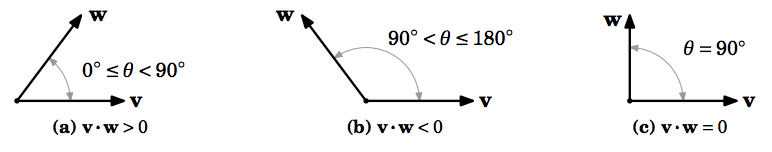
\includegraphics[width=0.7\textwidth]{img/fig-6-dot-product.jpg}
\end{figure}
\end{nota}
\end{definizione}
\begin{definizione}
  La funzione di costo viene espressa anche come:
  \[\theta^Tx^{(i)} = p^{(i)} \cdot \lVert \theta \rVert\]
  \begin{figure}[H]
    \centering
    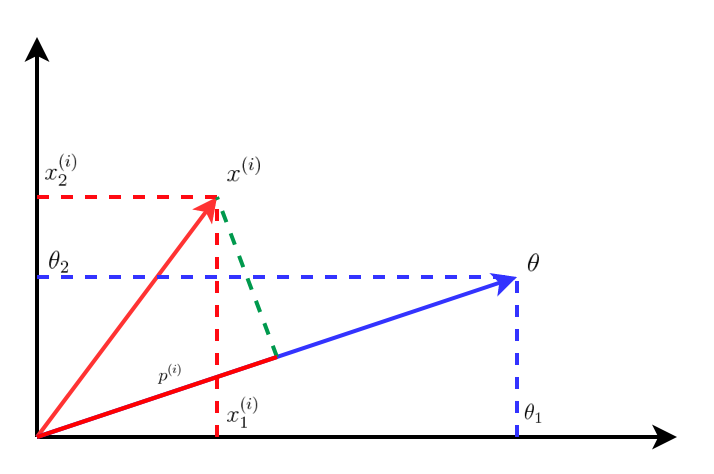
\includegraphics[width=0.7\textwidth]{img/fig-7-dot-product-in-svm.png}
\end{figure}
\end{definizione}
\begin{definizione}
  La funzione ci costo si può esprimere come:
  \[min_\theta \, {1 \over 2 } \lVert \theta \rVert^2 \]
  % <![CDATA[
\begin{align*}
p^{(i)} \cdot \lVert \theta \rVert &\geq 1 \text{, if } y^{(i)}=1 \\
p^{(i)} \cdot \lVert \theta \rVert &\leq -1 \text{, if } y^{(i)}=0
\end{align*} %]]>
\begin{nota}
Dove $p^{(i)}$ è la proiezione di $x^{(i)}$ sul vettore $\theta$.
\end{nota}
\end{definizione}
  \begin{esempio}
    Se il numero di classificazioni è 2 e $\theta_0 = 0$:
    \[min_\theta \, {1 \over 2 } (\theta_1^2 + \theta_1^2) = {1 \over 2 } \sqrt{(\theta_1^2 + \theta_1^2)}^2 =  {1 \over 2 } \lVert \theta \rVert^2 \tag{12} \label{12}\]
  \end{esempio}
Consideriamo due confini decisionali (A e B), e i loro corrispettivi parametri perpendicolari ($\theta_A$ e $\theta_B$). Se scegliessimo $\theta_0 = 0$ tutti i corrispettivi confini decisionali passerebbero per l'origine.
  \begin{figure}[H]
    \centering
    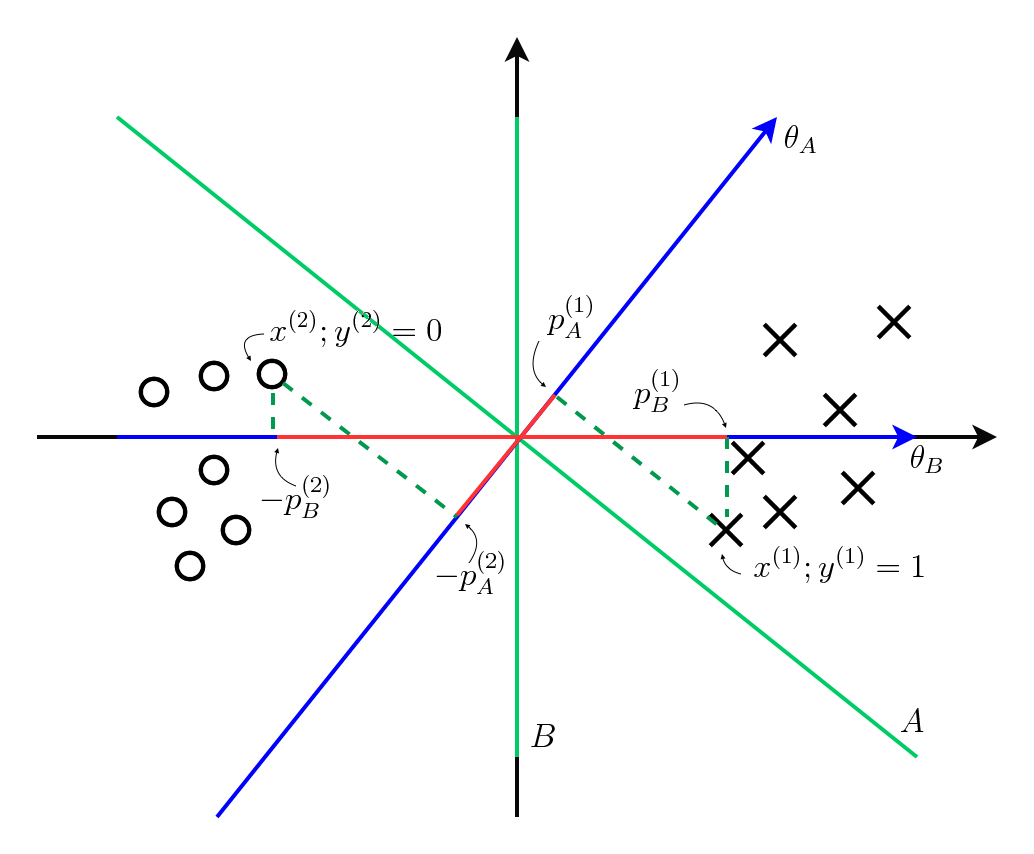
\includegraphics[width=0.7\textwidth]{img/fig-8-choosing-large-margin.png}
\end{figure}
\section{Esempi}
\textbf{Nell'esercitazione ogni $\vec{w}\cdot\vec{x}$ è da calcolarsi come
  $\vec{w}^T\cdot\vec{x}$.} 
\begin{definizione}
  Definiamo \textbf{iperpiano} su uno spazio euclideo a $n$ dimensioni come un
  sottoinsieme piatto di $n-1$ dimensioni che divide lo spazio in due parti non
  connesse. \\
  È quindi un luogo di punti che soddisfa:
  \[\vec{w}\cdot\vec{x}+b=0\]
  Ovviamente:
  \begin{itemize}
    \item in una dimensione è un punto
    \item in due dimensioni una retta
    \item in tre dimensioni un piano
    \item in più di tre dimensioni si usa direttamente il termine iperpiano
  \end{itemize}
  Nel caso a due dimensioni, per esempio, si ha che:
  \[\vec{w}\cdot\vec{x}+b=0\]
  (che in due dimensioni è la forma implicita di una retta) corrisponde a:
  \[w_0x+w_1y+b=0\]
  ovvero:
  \[w_1y=-w_0x-b\]
  Isolo quindi $y$:
  \[y=-\frac{w_0}{w_1}x-\frac{b}{w_1}\]
  e avendo:
  \begin{itemize}
    \item $m=-\frac{w_0}{w_1}$ come coefficiente angolare
    \item $q=-\frac{b}{w_1}$ come ordinata origine della retta, il punto di
    intercetta 
  \end{itemize}
  ottengo la classica equazione della retta, in forma esplicita:
  \[y=mx+q\]
  Quindi $\vec{w}\cdot\vec{x}+b$ assegna una sorta di ``punteggio''.

\end{definizione}
\begin{esempio}
  Preso $\vec{w}=(-0.4,-1)$ e $b=9$ si studino i punti $A(1, 3)$, $B(3, 5)$ e
  $C(5, 7)$.\\
  Si ottiene:
  \begin{itemize}
    \item per $A$, con $\vec{x}=(1, 3)$, si ha $\vec{w}\cdot\vec{x}+b=5.6$
    \item per $B$, con $\vec{x}=(3, 5)$, si ha $\vec{w}\cdot\vec{x}+b=2.8$
    \item per $C$, con $\vec{x}=(5, 7)$, si ha $\vec{w}\cdot\vec{x}+b=0$
  \end{itemize}
  Avendo che $C$ giace sull'iperpiano (l'equazione è nulla) e gli altri punti,
  essendo in due dimensioni e quindi avendo a che fare con una retta, sono sotto
  la retta ($A$ più lontano di $B$ avendo ``punteggio'' maggiore).
\end{esempio}
Con il percettrone si vedeva se i punti erano linearmente separabili (trovando
un iperpiano che separava) con SVM si cerca l'iperpiano ottimo per separare i
punti.
\begin{esempio}
  Sia data una funzione d'ipotesi (che definisce un'ipotesi in $H$) tale che:
  \[h(\vec{x}_i=
    \begin{cases}
      +1&\mbox{se }\vec{w}\cdot\vec{x}_i+b\geq 0\\
      -1&\mbox{se }\vec{w}\cdot\vec{x}_i+b< 0
    \end{cases}
  \]
  ovvero:
  \[h(\vec{x_i}=sign(\vec{w}\cdot\vec{x}_i+b)\]
  quindi i valori positivi sono sopra etichettati come positivi e i negativi
  come  negativi.\\
  Siano dati:
  \begin{itemize}
    \item $\vec{w}=(0.4, 1)$
    \item $b=-9$
    \item $A(8, 7)$ e $B(1, 3)$
  \end{itemize}
  Si ha:
  \begin{itemize}
    \item per $A$, che è sopra l'iperpiano:
    \[\vec{w}\cdot\vec{x}_i+b=0.4\cdot 8+1\cdot 7-9=1.2\]
    quindi è etichettato come positivo
    \item per $B$, che è sotto l'iperpiano:
    \[\vec{w}\cdot\vec{x}_i+b=0.4\cdot 1+1\cdot 3-9=-5.6\]
    quindi è etichettato come negativo
  \end{itemize}
  Ma non si è detto nulla sulla scelta dell'iperpiano, ne in termini di calcolo
  ne in termini studio della sua qualità.
\end{esempio}
Ci serve quindi una misura di confidenza per la classificazione usando i
\textbf{margini}. \\
Abbiamo quindi il punteggio $\beta$ dato da:
\[\beta=\vec{w}\cdot\vec{x}+b\]
e perché tale punteggio sia utile ci serve anche la classe di appartenenza
$y$. Si ha quindi:
\[f=y\cdot\beta\implies f=y\cdot(\vec{w}\cdot\vec{x}+b)\]
avendo ottenendo il \textbf{margine funzionale} $f$ tale che:
\begin{itemize}
  \item $f$ è positivo se la classificazione è corretta
  \item $f$ è negativo se la classificazione non è corretta
\end{itemize}
Inoltre:
\begin{itemize}
  \item se si ha $y=1$ allora affinché il margine funzionale sia ampio (cioè,
  affinché la nostra previsione sia sicura e corretta), allora abbiamo bisogno
  che $\vec{w}\cdot\vec{x}+b$ sia un numero positivo grande 
  \item se si ha $y=-1$ allora affinché il margine funzionale sia grande, allora
  abbiamo bisogno che $\vec{w}\cdot\vec{x}+b$ sia un grande numero negativo 
\end{itemize}

Per una certa osservazione $i$ si ha quindi (usiamo la dicitura $\hat{gamma}$ al
posto di $f$ per il margine funzionale):
\[\hat{\gamma}^{(i)}=y^{(i)}(\vec{w}\cdot\vec{x}+b)\]
e quindi per tutti i dati si cerca:
\[\hat{\gamma}=\min \hat{\gamma}^{(i)}\]
Ma si ha ancora un problema: dipende dalla scala. Se a $\vec{w}$ sostituiamo,
ad esempio, $2\vec{w}$ e a $b$ sostituiamo $2b$ si ha che la classificazione
fatta con $sign(\vec{w}\cdot\vec{x}_i+b)$ resta la medesima (anche perché
l'iperpiano resta lo stesso, avendo dipendenza lineare). D'altro canto il
margine funzionale aumenta all'aumentare dei due valori (aumentando lo score) e
quindi si ha una ``falsa'' confidenza (sembrando due volte più confidente quando
è tutto uguale in realtà, dall'iperpiano alla classificazione).\\
Si introduce quindi il \textbf{margine geometrico}, dividendo il margine
funzionale per la norma di $\vec{w}$:
\[\hat{\gamma}^{(i)}=y^{(i)}\left(\frac{\vec{w}}{\norm{\vec{w}}}
    \cdot\vec{x}^{(i)}+\frac{b}{\norm{\vec{w}}}\right)\]
si ha quindi un invaiante rispetto al fattore di scala, a differenza del margine
funzionale (con la divisione per la norma semplifico eventuali fattori
moltiplicativi costanti).\\
Anche in questo caso cerco il minimo:
\[\hat{\gamma}=\min \hat{\gamma}^{(i)}\]
Con SVM si cerca l'iperpiano ottimo ovvero che massimizza il margine per
entrambe le classi considerate nel training set, rendendo massima la distanza
tra i punti più vicini di ogni classe, minimizzando il margine geometrico di
ogni esempio. Si trovano i support vector dove giacciono i più vicini punti
all'iperpiano per le due classi. Il risultato dell'ottimizzazione per SVM è
trovare il gap maggiore che ci separa da tutte le classi contemporaneamente
\begin{figure}[H]
  \centering
  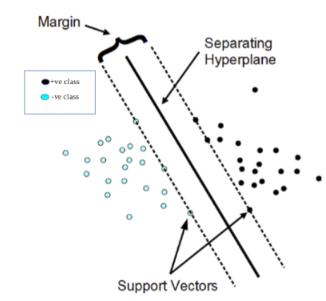
\includegraphics[scale = 0.7]{img/svm.jpg}
  \caption{Visualizzazione di SVM}
  \label{fig:svm}
\end{figure}
Se non si può separare positivi dai negativi (o un training set non linearmente
separabile) in uno spazio di bassa dimensione
utilizzando un iperpiano, bisogna mappare tutto in uno spazio dimensionale
superiore dove è possibile separarli, tramite i \textbf{metodi kernel}. Tramite
una funzione $\phi$ si passa lo spazio d'input in uno nuovo, detto
\textbf{feature space}, a dimensione maggiore, dove i punti sono linearmente
separabili.  
\begin{esempio}
  Dato $[x^{(1)}, x^{(2)}]$ si ha:
  \[\phi([x^{(1)}, x^{(2)}])=[x^{(1)2}, x^{(2)2}, x^{(1)}x^{(2)}]\]
  facendo, in questo esempio, il quadrato delle due componenti e il loro
  prodotto, da due dimensioni passo a 3.
\end{esempio}
\begin{definizione}
  Dato uno spazio delle istanze $X$ e un feature space $F$ si ha che una
  funzione $k$:
  \[k_X\to X\times X\to\mathbb{R}\]
  è detta kernel valido sse esiste una \textit{feature map} $\phi$:
  \[\phi:X\to F\]
  tale che:
  \[k(x, z)=\langle\phi(x),\phi(z)\rangle,\,\,\,\forall\, x, z\in X\]
  avendo quindi che posso rappresentare $k$ tramite un prodotto interno di
  feature risultate dal mapping definito da $\phi$.\\
  La funzione $k$ ha quindi come argomenti due vettori senza restrizioni,
  potendo mappare un ampio spettro di entità (documenti, proteine etc$\ldots$),
  può quindi essere penata come una \textbf{funzione si similarità} (pensata
  come prodotto euclideo), dicendo
  quanto sono simili gli oggetti della funzione kernel.\\
  Avendo il prodotto interno scalare si ha anche la norma, dando prova della
  lunghezza del vettore, e avendo anche la \textbf{distanza} tra due vettori
  nello spazio, che all'inverso è una misura di similarità.
\end{definizione}
\begin{definizione}
  Definiamo \textbf{kernel matrix}, detta anche \textbf{gram matrix}, dato un
  kernel $k$ e un insieme 
  $S=x_1, x_2,\ldots x_n$, come una matrice dove ogni componente è:
  \[G_{i, j}=\langle\phi(x_i),\phi(x_j)\rangle_{\mathcal{H}}=k(x_i, x_j)\]
\end{definizione}
Molti algoritmi interagiscono coi dati tramite prodotti scalari per questo sono
importanti le funzioni kernel. Per definizione di kernel posso quindi sostituire
un prodotto interno tra due vettori con la funzione kernel definita sui quei due
vettori, spostandomi in una dimensione maggiore per il feature space e ottenendo
un valore di similarità tra i due oggetti. 
\begin{esempio}
  Vediamo un esempio di funzione kernel. \\
  Siano dati:
  \begin{itemize}
    \item $\vec{x}=(x_1, x_2)$
    \item $\vec{z}=(z_1, z_2)$
    \item $dim=2$
  \end{itemize}
  Si ha quindi:
  \[(\vec{x}\cdot\vec{z})^2=(x_1z_1+x_2z_2)^2
    =(x_1^2x_2^2+x_2^2z_2^2+2x_1z_1x_2z_2)\]
  \[=\langle\left(x_{1}^{2}, x_{2}^{2}, \sqrt{2} x_{1}
      x_{2}\right),\left(z_{1}^{2}, z_{2}^{2}, \sqrt{2} z_{1}
      z_{2}\right)\rangle=\langle\phi(\vec{x}),\phi(\vec{z})\rangle\]
  Avendo ottenuto le feature. Quindi la funzione iniziale è rappresentabile come
  il prodotto interno tra le due feature, in modo implicito.\\
  Avendo quindi:
  \[\phi(x_1, x_2)=(x_1^2, x_2^2,\sqrt{2}x_1x_2\]
  \[\phi(xz_1, z_2)=(z_1^2, z_2^2,\sqrt{2}z_1z_2\]
  passando a $dim=3$.
\end{esempio}
Tra i tipo di kernel si segnala quello gaussiano:
\[ k(\mathbf{x}, \mathbf{z}) =\exp \left(-\frac{\|\mathbf{x}-
      \mathbf{z}\|^{2}}{2 \sigma^{2}}\right) 
  =\exp \left(-\frac{\mathbf{x}^{\mathbf{T}} \mathbf{x}-\
      mathbf{2} \mathbf{x}^{\mathbf{T}} \mathbf{z}+
      \mathbf{z}^{\mathbf{T}} \mathbf{z}}{2 \sigma^{2}}\right)\]
La strategia di kernel di un algoritmo è che ogni volta che si trova un prodotto
interno di feature si ha che questo è uguale al kernel nello spazio
originale. Non serve conoscere il mapping se il kernel è valido e posso quindi
procedere direttamente con la sostituzione.
\begin{definizione}
  Un metodo è detto \textbf{kernelizzato} se il prodotto interno delle sue
  feature può essere valutato da una qualunque funzione kernel nello spazio di
  rappresentazione originale.
\end{definizione}
Le distanze e le differenze sono state questioni importanti nel machine
learning e nel riconoscimento di modelli per molti anni, portando a molti
algoritmi noti diversi e domande importanti.\\
La distanza tra oggetti nello spazio delle feature è definita da:
\[d(x, x_2)=\norm{\phi(x)-\phi(x_2)}^2_{\mathcal{H}}\]
denotando con $\mathcal{H}$ lo spazio del prodotto interno dove le feature sono
rappresentate dal mapping:
\[\phi:X\to \mathcal{H}\]
Si ha quindi per la distanza, estendendo la norma:
\[
  \left\|\Phi\left(x_{1}\right)-\Phi\left(x_{2}\right)\right\|_{\mathcal{H}}^{2}
  =<\Phi\left(x_{1}\right)-\Phi\left(x_{2}\right),
    \Phi\left(x_{1}\right)-\Phi\left(x_{2}\right)>\]
    \[
  =<\Phi\left(x_{1}\right), \Phi\left(x_{1}\right)>-2<\Phi
  \left(x_{1}\right), \Phi\left(x_{2}\right)>+<\Phi\left(x_{2}\right),
  \Phi\left(x_{2}\right)>
\]
e con la notazione kernel, avendo sostituito con un kernel valido $k$, ottenendo
una riscrittura della distanza tra due feature, kernelizzando la distanza tra
due input:
\[\left\|\Phi\left(x_{1}\right)-\Phi\left(x_{2}\right)\right\|_{\mathcal{H}}^{2}
  =k(x_1, x_1)-2k(x_1, x_2)+k(x_2, x_2)\]
\textbf{Si hanno liste di funzioni kernel verificate.}